
En el faro de los automóviles se acostumbra poner, además del espejo principal \textit{E}$_{1}$, otro espejo pequeño esférico \textit{E}$_{2}$ (véase figura de esta pregunta). Este espejo auxiliar debe colocarse de tal manera que los rayos luminosos que salen de la fuente \textit{S} y que inciden en él se reflejen sobre sí mismos, para que el máximo de luz de esta fuente se transforme en ``luz paralela'', al salir del faro. Sabiendo que \textit{E}$_{1}$ tiene 16,0 cm de radio y el radio de \textit{E}$_{2}$ es igual a 2,0 cm, las distancias \textit{SM} y \textit{SN}, mostradas en la figura, deben valer, respectivamente:

    \textit{a}) $8.0 \text{ cm}$ y $1.0 \text{ cm}$. 
    \textit{b})  $16.0 \text{ cm}$ y $2.0 \text{ cm}$.
    \textit{c})  $16.0 \text{ cm}$ y $1.0 \text{ cm}$.
    \textit{d})  $8.0 \text{ cm}$ y $4.0 \text{ cm}$.
    \textit{e})  $8.0 \text{ cm}$ y $2.0 \text{ cm}$.

\begin{figure}[h!]
    \centering
    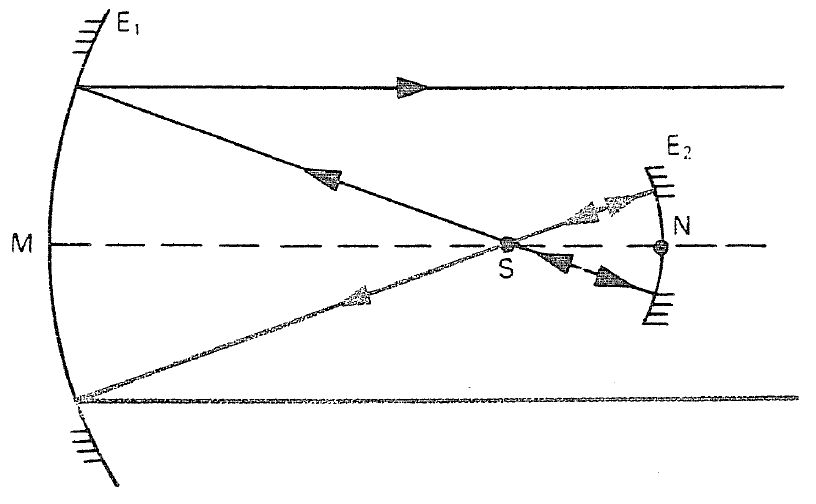
\includegraphics[scale=0.38]{enunciados/alvarenga_p653_11.png}
    \caption{Alvarenga p. 653 - Ejercicio 11}
\end{figure}